
\section{Analysis}\label{sec:analysis}

Minimal plots using summary \ac{JSON}:
\begin{itemize}
\item Barchart (mean, max, min, q1, q2, q3, q4) of bitrate
\item Barchart (mean, max, min, q1, q2, q3, q4) of buffer
\item Barchart (mean, max, min, q1, q2, q3, q4) of stall duration
\item Barchart of number of switches (up), number of switches (down),  number of stalls
\end{itemize}


Advanced plots:
%\begin{itemize}
%\item  Buffer vs. time, buffer+playback+downloaded playtime vs. time
%\item Bitrate vs. time
%\item \ac{ECDF} of bitrate OR (barchart?) percentile-min-max-mean comparison
%\item YouTube vs. AStream of bitrate
%\item Time spent on each quality level YouTube vs. AStream
%\item (barchart?) num. Switches, num. Stalls YouTube vs. AStream
%\end{itemize}

\begin{itemize}
\item Bitrate
\begin{itemize}
\item Bitrate (Kbps) vs. Time (s), YoMo and AStream
\item \ac{ECDF} of bitrate (Kbps), YoMo and AStream
\end{itemize}
\item Buffer
\begin{itemize}
\item Buffer (s) vs. Time (s), YoMo and AStream 
\item Buffer (s) + playback (s) + downloaded playtime (s) vs. Time (s), YoMo
\item Buffer (s) + playback (s) + downloaded playtime (s) vs. Time (s), AStream
\end{itemize}
\item Quality levels
\begin{itemize}
\item Time spent at each (s) vs. Level (name), barchart, YoMo and AStream
\item Switch and Stalls
\item Num. up switches, num. Down switches, num. Stalls, YoMo and AStream
\end{itemize}
\end{itemize}

\begin{figure} [h!]
\caption{Sample plots.}
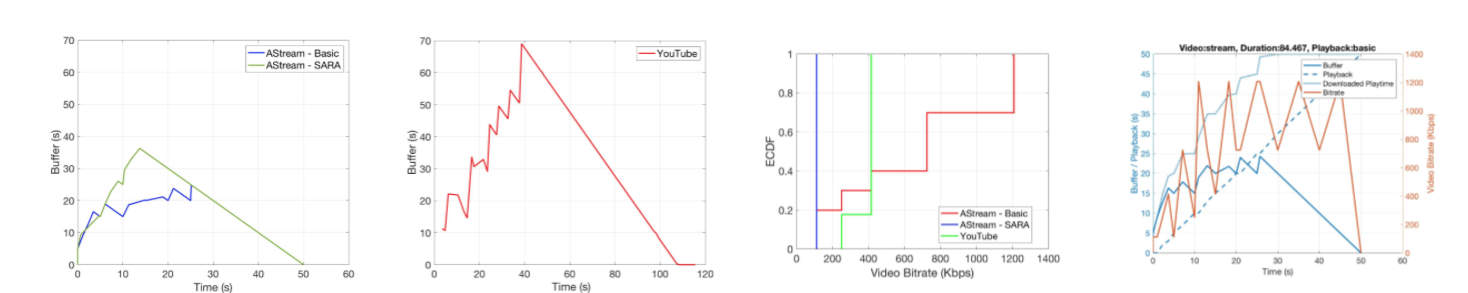
\includegraphics[width=\textwidth]{graphics/sampleplots}
\label{fig:sampleplots}
\end{figure}

\begin{figure} [h!]
\caption{Flo notes.}
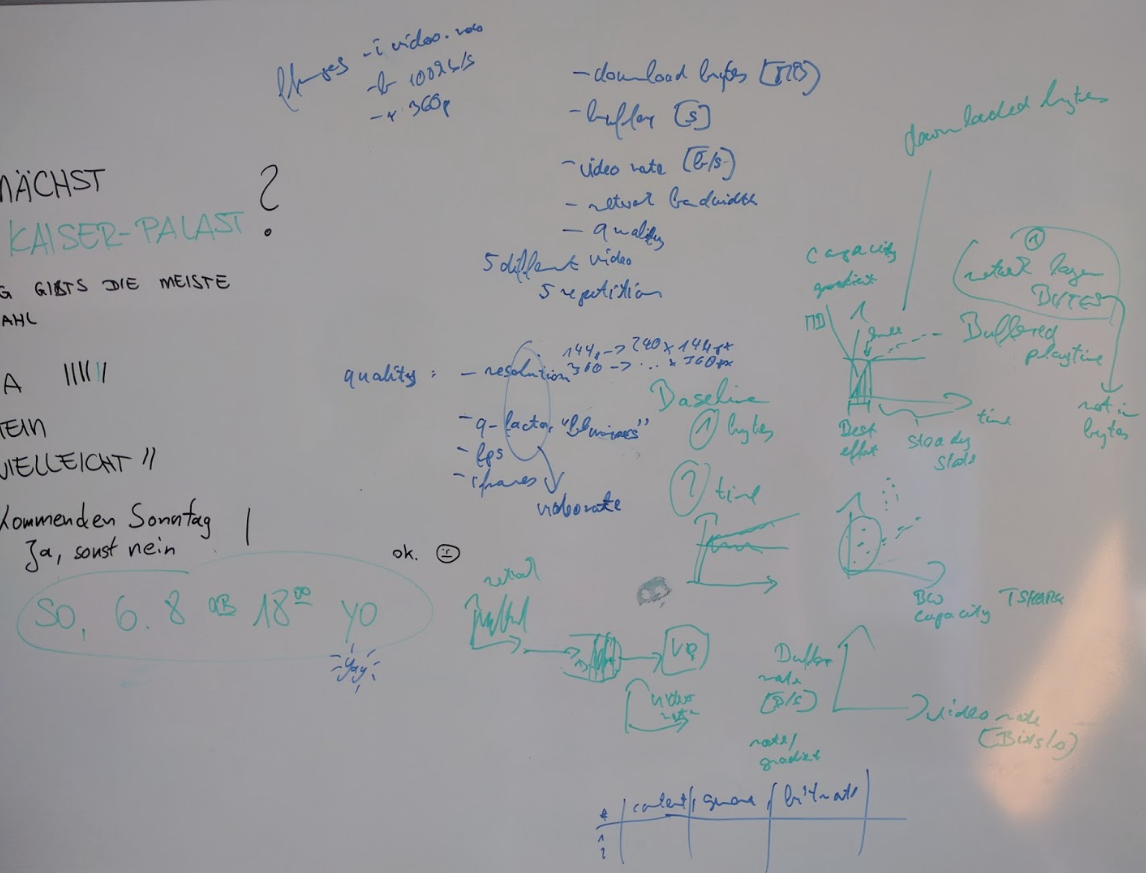
\includegraphics[width=\textwidth]{graphics/flonotes}
\label{fig:flo notes}
\end{figure}
